Todo lo anterior lleva al punto crítico en donde se encuentran los contenedores y
tecnologías como Docker actualmente: ¿cómo se automatiza el despliegue? ¿Cómo se
realizan escalados automáticos? ¿Cómo se guardan recursos, se conservan y se
reutilizan más tarde? Bienvenidos a la orquestación de contenedores.

Actualmente las herramientas de orquestación están en boga y son la clave del
desarrollo basado en contenedores. Ofrecen una gran polivalencia y flexibilidad
a la hora de desplegar aplicaciones a lo largo de clústers distribuidos de una
forma relativamente sencilla y accesible.

Herramientas como Kubernetes, Minikube, AWS EKS o Docker Swarm son de las más
sonadas y utilizadas actualmente. El primero de ellos es actualmente el más usado
a nivel mundial. Kubernetes es una herramienta de código abierto diseñada por Google
que permite orquestar contenedores a lo largo de una red distribuida de nodos. Minikube
por su parte es una versión local de Kubernetes con las mismas características,
muy útil para desplegar aplicaciones en entornos locales y hacer pruebas antes
de un despliegue global. AWS EKS es la solución nativa de Amazon para su servicio
en la nube de orquestación. Se basa en Kubernetes y permite realizar una gestión
individualizada de los contenedores para ajustar el pago y los recursos destinados.
Finalmente, Docker Swarm es la solución nativa de Docker para la orquestación de
contenedores. Se gestiona con el propio CLI de Docker y, aunque no es tan popular
como otras herramientas, está ganando fuerza debido a su gran facilidad de uso.

\subsubsection*{¿Por qué es importante la orquestación de contenedores?}
Es fundamental intentar vislumbrar el porqué han ganado tanto peso estas
herramientas de orquestación ya que es la clave de muchas empresas. La organización
en contenedores automatiza la implementación, la gestión, la escalabilidad y la
conexión en red de los contenedores. Empresas que necesiten implementar y
gestionar cientos o miles de \textit{hosts} usando contenedores Linux se benefician
directamente de la orquestación de contenedores \cite{QueEsOrganizacion}.

En particular, estas tecnologías han visto un gran auge con la aparición de los
microservicios organizados en contenedores. Con ellas se pueden desplegar más
instancias de un microservicio si la carga del sistema es elevada o reducir los
contenedores según sea la demanda. Por otra parte, los microservicios son muy
útiles en la gestión de los ciclos de vida de los contenedores, en particular 
para los equipos de DevOps: una integración correcta en los flujos de trabajo de
CI/CD permiten definir la base de las aplicaciones nativas en la nube.

Es por ello por lo que las tecnologías de orquestación han proliferado y
permiten definir automatizar y gestionar muchas tareas \cite{QueEsOrganizacion}:

\begin{itemize}
    \item Preparación e implementación.
    \item Configuración y programación.
    \item Asignación de recursos.
    \item Disponibilidad de contenedores.
    \item Ajusta o eliminación de contenedores según la carga del sistema.
    \item Equilibrio de cargas y enrutamiento de tráfico.
    \item Supervisión del estado de los contenedores.
    \item Configuración de aplicaciones en función del contenedor en que se
          vayan a ejecutar.
    \item Protección de las interacciones entre contenedores.
\end{itemize}

Con todas estas tareas automatizadas, es más sencillo gestionar aplicaciones
distribuidas. Todo esto es necesario debido a la naturaleza ligera y efímera
de los contenedores, en donde el ciclo de vida de alguno de ellos puede llegar
a ser de unos pocos segundos (como en microservicios). Así, la orquestación viene
a ofrecer los siguientes beneficios \autocite{ContainerOrchestration}:

\begin{itemize}
    \item Simplicidad en las operaciones, el gran beneficio de la orquestación:
          según lo expuesto anteriormente, las aplicaciones basadas en contenedores
          pueden introducir una gran complejidad y generar muchísimos datos. Con
          la orquestación es más simple gestionarlo.
    \item Resiliencia, permitiendo el reinicio y escalado de los contenedores 
          necesarios según se necesite de forma automática.
    \item Seguridad, ya que se reduce el error humano.
\end{itemize}

\subsubsection{Herramientas de orquestación}
\subsubsection*{Kubernetes}

\begin{figure}[H]
    \centering
    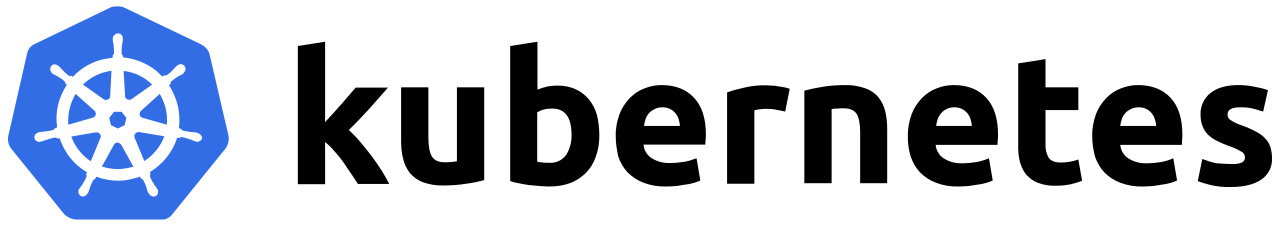
\includegraphics[width=\linewidth]{pictures/kubernetes-logo.png}
    \caption{Logo de Kubernetes \autocite{ArchivoKubernetesLogo}.}
    \label{fig:k8s-logo}
\end{figure}
Kubernetes es actualmente la herramienta de orquestación más utilizada por las
compañías que basan sus aplicaciones en contenedores \autocite{ContainerAdoptionTrends}.
Fue una herramienta de código libre creada por Google y donada a la \textit{Cloud Native Computing
Foundation}, quien lo gestiona ahora.

Dado que los contenedores son una buena manera de desplegar aplicaciones, la gestión
en entornos de producción se cede a herramientas como K8s que se aseguran de que
no exista tiempo de \textit{downtime} (K8s son las siglas de ``Kubernetes'', donde
el 8 representa las ocho letras entre la `K' y la `s'). Por ejemplo, si un
contenedor se cae y no ofrece servicio, automáticamente otro se crea y se levanta
y suple al anterior \autocite{WhatKubernetes}.

K8s ofrece un \textit{framework} para poder ejecutar sistemas distribuidos de
forma resiliente. Gestiona automáticamente el escalado y el control de fallos
de la aplicación, ofrece patrones de despliegue y más opciones, entre las
que se destacan \autocite{WhatKubernetes}:

\begin{itemize}
    \item Descubrimiento de servicios y balanceo de carga: mediante el uso de
          direcciones DNS o direcciones IP, K8s puede exponer un contenedor
          a la red. Si por un casual el tráfico es elevado, aprovechando el
          mecanismo anterior se puede redirigir automáticamente a un contenedor
          con poca carga o que pueda servir la operación de una forma más
          eficaz.
    \item Orquestación del almacenamiento: Kubernetes permite gestionar el
          almacenamiento local, en la nube o en proveedores para los contenedores
          que lo necesiten.
    \item \textit{rollouts} y \textit{rollbacks}: mediante la descripción de
          los estados en los que se pueden encontrar los contenedores (como el
          estado ``deseable''), Kubernetes puede modificar el estado para
          alcanzar dicho estado deseable o bien volver a un estado controlable.
          Un ejemplo sería el despliegue de nuevos contenedores, eliminar los
          ya existentes y adoptar sus recursos para continuar desde el
          estado en que se dejó.
    \item Gestión de los recursos: se puede configurar un clúster de Kubernetes
          para que use una cantidad específica de CPU y de RAM y automáticamente
          se distribuirán los servicios para hacer el uso más eficiente posible
          de los recursos.
    \item Autocuidado: si un contenedor falla, se reinicia; si no funciona como
          se espera, se reemplaza; si no hay respuesta en un plazo de tiempo, se
          finaliza. Todo esto se hace de forma transparente al usuario y nunca se
          ofrecen servicios que todavía no estén disponibles.
    \item Gestión de ``secretos'' y configuraciones: K8s facilita la gestión
          de información sensible como contraseñas, claves OAuth, etc., permitiendo
          la actualización de dichos valores sin necesidad de desplegar de nuevo
          la aplicación y sin exponer dicha información al exterior.
\end{itemize}

Sin embargo, es fundamental tener en cuenta qué operaciones nunca va a realizar
Kubernetes y que lo diferencian de otras soluciones o alternativas. Por una parte,
Kubernetes no es una PaaS (\textit{Platform as a Service}) tradicional. Esto se
debe a que K8s no es monolítico y aunque comparte muchas características comunes
con un PaaS otras son libres, configurables y se ajustan por el usuario.

Por otra parte, las aplicaciones no están limitadas en principio: si se puede
ejecutar en un contenedor debería funcionar correctamente en Kubernetes. Además,
Kubernetes en ningún momento despliega código fuente o construye una aplicación.
Esto se aplica directamente en los entornos de CI/CD, en donde los requisitos y
las funciones se determinan por el equipo de trabajo.

En lo referente a servicios a nivel de aplicación, Kubernetes no ofrece mecanismos
como \textit{middlewares}, \textit{frameworks} de procesamiento de datos, 
bases de datos, cache o sistemas de almacenamiento en clústers de forma nativa.
Dichos componentes se pueden ejecutar en K8s pero se han de configurar mediante
mecanismos externos.

Un factor muy importante es que no hay mecanismos de registro, monitorización o
alertas: existen ciertas integraciones como prueba de concepto y mecanismos de
recolección y exportación de métricas de funcionamiento.

\subsubsection*{¿Cómo funciona Kubernetes?}
Cuando se despliega a Kubernetes, se crea un clúster. Un clúster se compone de un
conjunto de máquinas (llamadas nodos) que ejecutan aplicaciones en contenedores.
Es requisito que cada clúster contenga al menos un único nodo.

Dicho nodo aloja lo que se conoce como ``\textit{pods}'', un conjunto de componentes
de la aplicación que se ejecutan en el nodo. Esto se apoya de un ``\textit{control plane}''
que gestiona los nodos y los \textit*{pods} en el clúster. Idealmente, en un
entorno de producción, este \textit{control plane} se ejecuta a lo largo de
múltiples equipos y un clúster se despliega en múltiples nodos, ofreciendo una
alta disponibilidad y tolerancia a fallos. Un entorno completo de Kubernetes
se muestra en la figura \ref{fig:k8s-cluster}:

\begin{figure}[H]
    \centering
    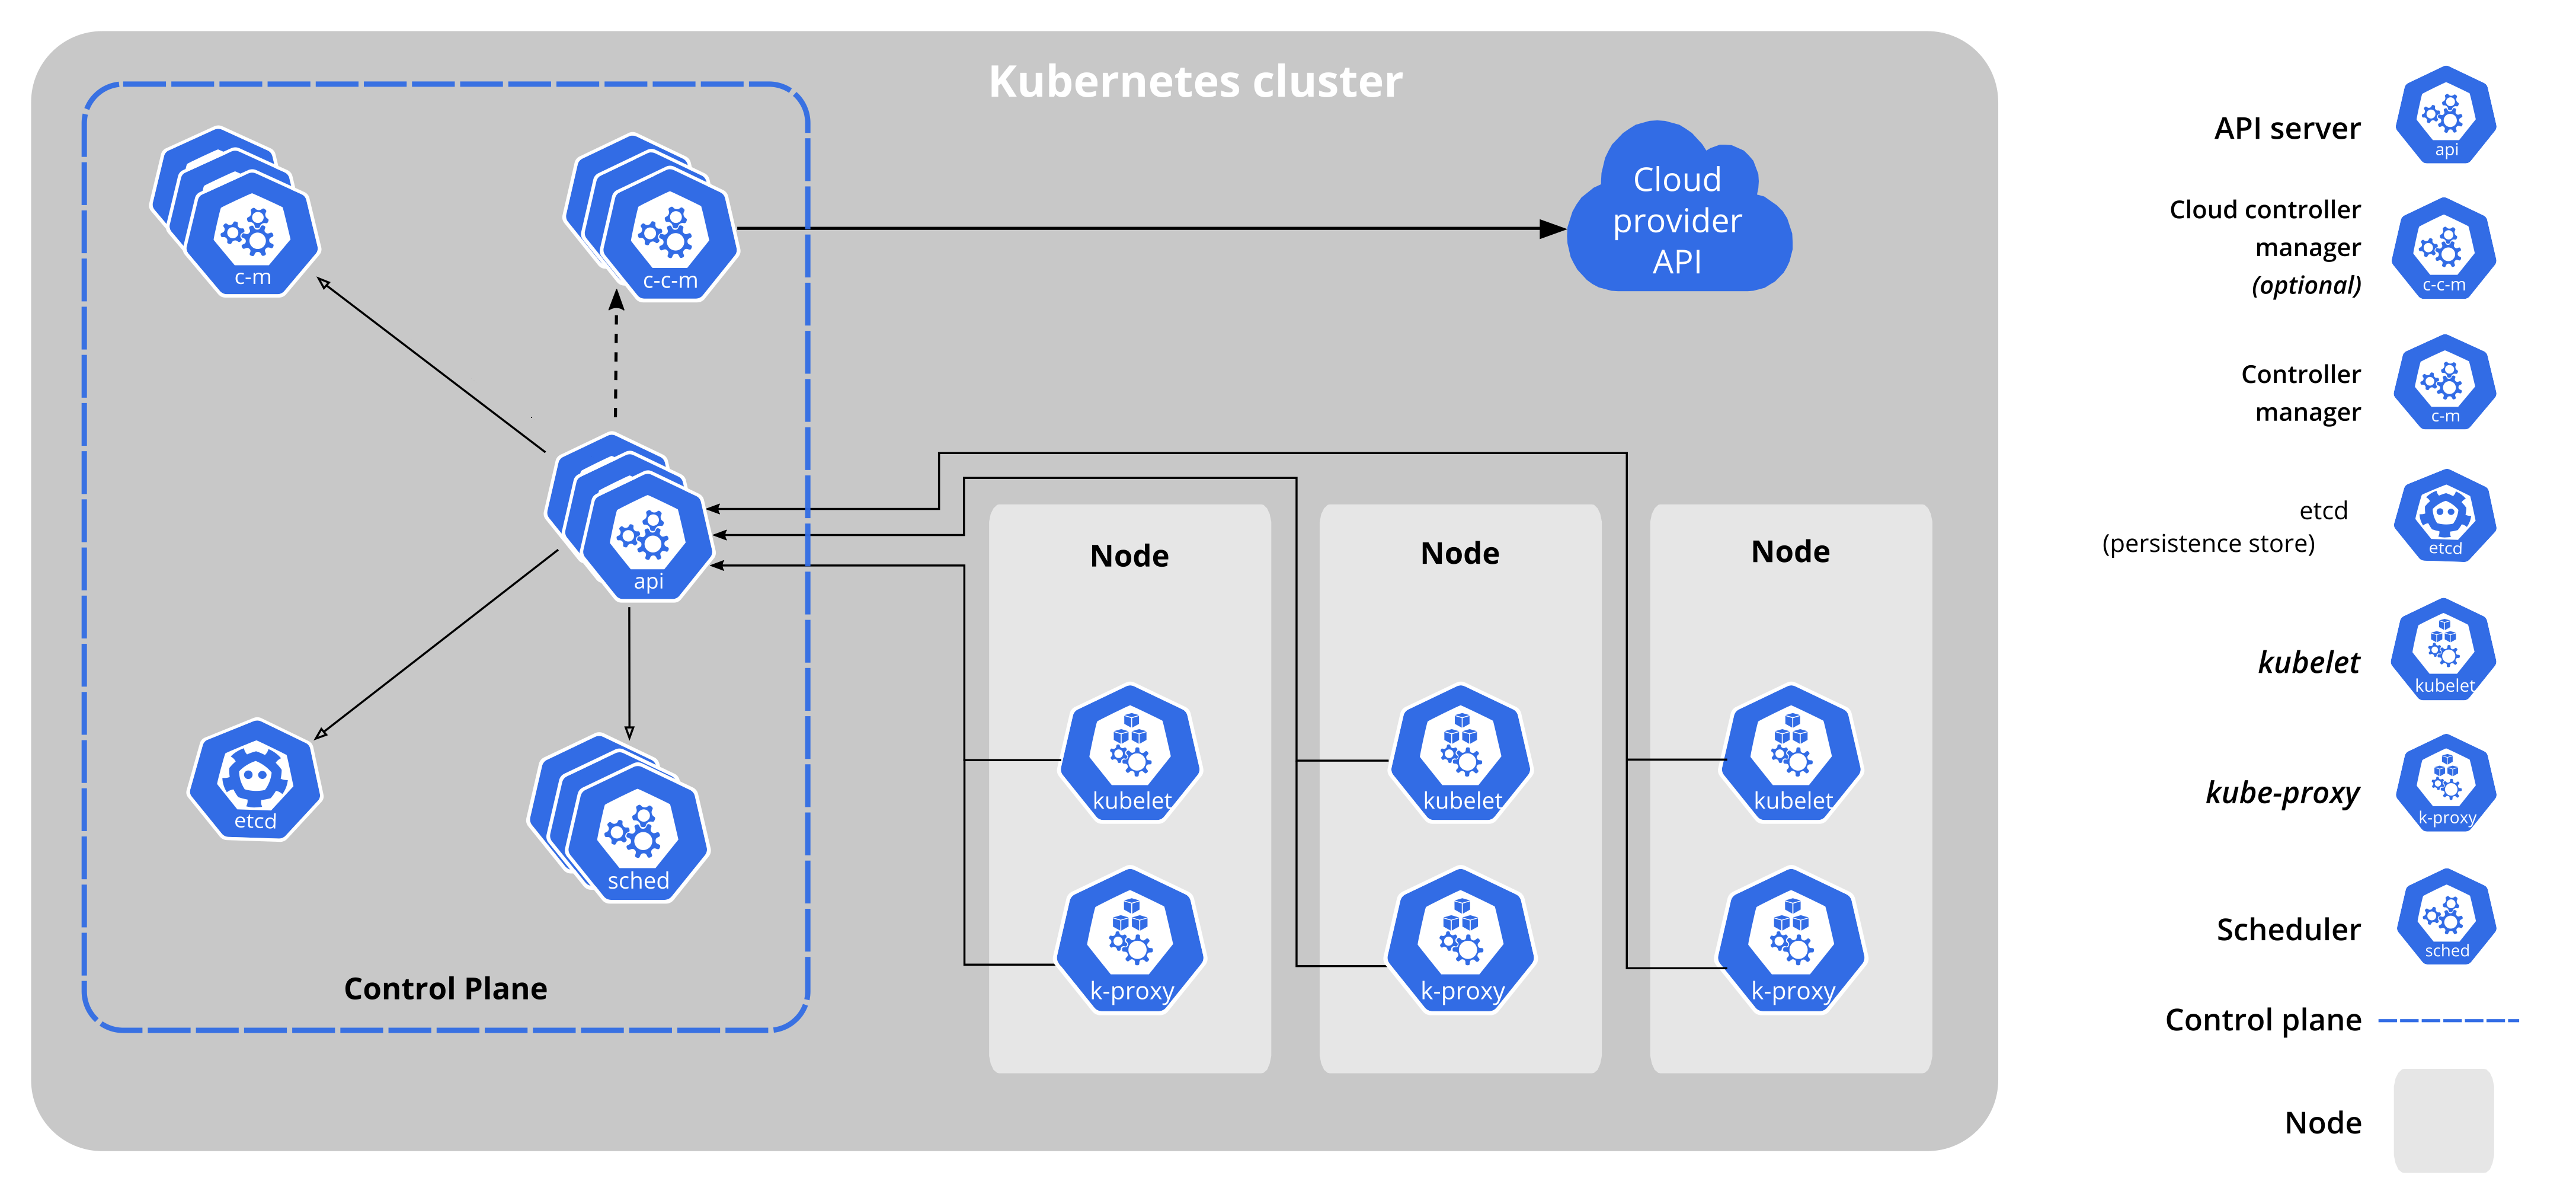
\includegraphics[width=\linewidth]{pictures/components-of-kubernetes.png}
    \caption{Componentes de Kubernetes \autocite{KubernetesComponents}.}
    \label{fig:k8s-cluster}
\end{figure}

\subsubsection*{El \textit{control plane} de Kubernetes}
Los componentes \textit{control plane} permiten tomar decisiones globales en
lo referente al clúster y detectar y responder a eventos que se den en el
clúster.

De entre todos los componentes que existen, algunos importantes son:

\begin{itemize}
    \item \texttt{kube-apiserver} es un componente que expone la API de
          Kubernetes. Está diseñado para escalar horizontalmente desplegando
          más instancias y se pueden ejecutar múltiples instancias para balancear
          la carga del sistema.
    \item \texttt{etcd} es un almacenamiento de alto rendimiento basado en
          clave--valor que se usa para almacenar los datos de los clústers.
    \item \texttt{kube-scheduler} monitoriza los \textit{pods} que se han creado
          sin ningún nodo asignado a él y planifica su ejecución y en qué nodo
          se ejecutarán. Para definirlo se tienen en cuenta factores como los
          requisitos individuales y grupales de recursos, las características
          del \textit{software}, \textit{hardware} y de seguridad, la localización
          de los datos, etc.
    \item \texttt{kube-controller-manager} ejecuta los procesos \texttt{controller}.
          Estos controladores se definen según en donde se vayan a ejecutar:
          \begin{itemize}
              \item Controladores de nodos que gestionan qué sucede cuando un nodo
                    se cae.
              \item Controladores de trabajo que gestionan cómo los \textit{pods}
                    ejecutan tareas.
              \item Controladores de los \textit{endpoints} que exponen dichos
                    \textit{endpoints} a los servicios que los necesiten.
              \item Controladores de cuentas y tokens para la gestión del acceso
                    a la API.
          \end{itemize}
    \item \texttt{cloud-controller-manager} es similar a \texttt{kube-controller-manager}
          con la diferencia de que está destinado a la gestión de los controladores
          según el proveedor \textit{cloud} que se esté usando.
\end{itemize}

\subsubsection*{Componentes de los nodos}
Estos componentes se ejecutan en cada nodo y son el entorno de ejecución real de
Kubernetes:

\begin{itemize}
    \item \texttt{kubelet} es un agente que se ejecuta en cada nodo del clúster y
          se asegura de que los contenedores se estén ejecutando en un \textit{pod}.
          Tomando los valores definidos en \texttt{PodSpecs} se asegura de que los
          contenedores descritos en esa especificación se estén ejecutando y
          no contengan fallos. Es importante tener en cuenta que \texttt{kubelet}
          solo gestiona contenedores creados dentro de Kubernetes.
    \item \texttt{kube-proxy} es un proxy de red que se ejecuta en cada nodo e
          implementa parte del concepto de servicio. Este componente gestiona las
          reglas de red de los nodos y aprovecha los mecanismos del sistema operativo
          para redirigir el tráfico. En otro caso, lo hace él mismo.
    \item \textit{Container runtime} es la capa de ejecución de los contenedores en
          sí. Aquí aparecen tecnologías como Docker, containerd, etc.
\end{itemize}

\subsubsection*{Ejemplo aplicación en Kubernetes}
Para completar esta sección, se va a exponer un ejemplo de cómo desplegar una
aplicación en Kubernetes basándose en la guía publicada en la documentación
oficial \autocite{UseServiceAccess}.

En este ejemplo se van a desplegar dos instancias de una aplicación ``Hello World'',
se va a crear un servicio que expone un puerto del nodo y se accederá a la
aplicación en ejecución.

\textit{Nota: se asume que se tiene instalada la herramienta de gestión de Kubernetes
\texttt{kubectl} y un servicio de Kubernetes local, como \texttt{minikube}.}

Lo primero será definir la aplicación de Kubernetes que queremos desplegar. Al
igual que con Docker Compose, la definición se basa en ficheros YAML (código \ref{lst:kubernetes}):

\begin{lstlisting}[style=kubernetes, caption={Configuración de una aplicación ``Hello World'' en Kubernetes.}, label={lst:kubernetes}]
apiVersion: apps/v1
kind: Deployment
metadata:
  name: hello-world
spec:
  selector:
    matchLabels:
      run: load-balancer-example
  replicas: 2
  template:
    metadata:
      labels:
        run: load-balancer-example
    spec:
      containers:
        - name: hello-world
          image: gcr.io/google-samples/node-hello:1.0
          ports:
            - containerPort: 8080
              protocol: TCP
\end{lstlisting}

En el fichero anterior se define, por una parte, la versión de la API de Kubernetes
que se quiere usar. A continuación, el tipo de aplicación que se quiere desplegar
(clave \texttt{kind}). Puede ser: \texttt{Pod}, \texttt{DaemonSet}, \texttt{Deployment}
o \texttt{Service}. Después aparece la definición de las especificaciones del
Pod que se va a desplegar. En este caso, se define un selector que va a ejecutar 
aplicaciones con una etiqueta ``\texttt{load-balancer-example}'', se van a tener
dos réplicas y se parte de una plantilla que define la etiqueta y el contenedor que
va a ejecutar, en este caso una aplicación NodeJS que se expone en el puerto 8080.

Con el fichero ya definido se despliega la aplicación en el clúster:

\begin{lstlisting}[style=bash, caption={}]
kubectl apply -f hello-application.yaml
\end{lstlisting}

Esto habrá creado el despliegue (\texttt{Deployment}) y el conjunto de réplicas que
contendrá los dos pods. Para obtener información sobre el despliegue:

\begin{lstlisting}[style=bash, caption={}]
kubectl get deployments hello-world
kubectl describe deployments hello-world
\end{lstlisting}

\begin{figure}[H]
    \centering
    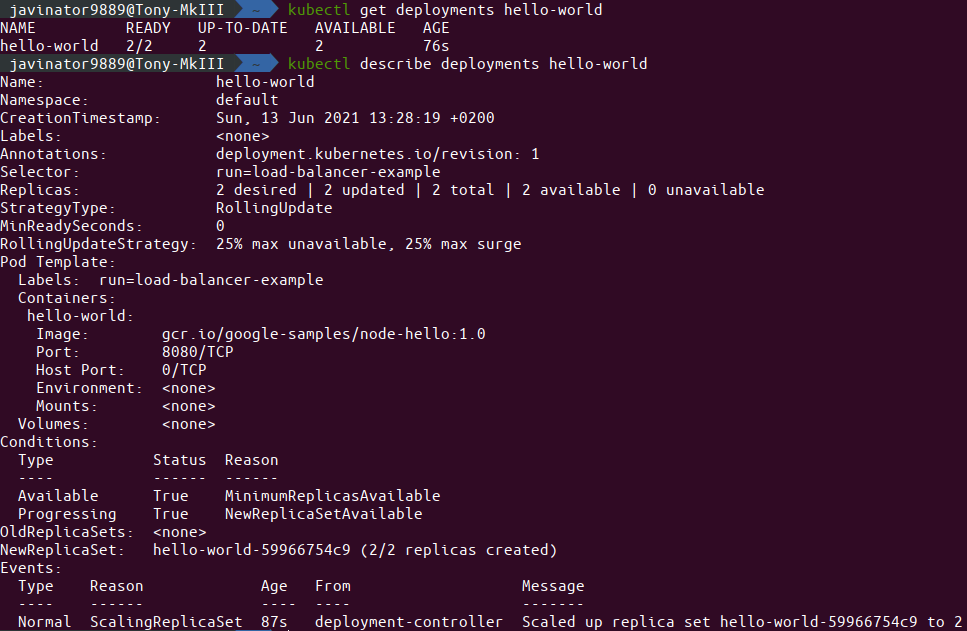
\includegraphics[width=.9\linewidth]{pictures/kubectl-deployments.png}
    \caption{Información sobre los despliegues en Kubernetes.}
    \label{fig:deployments}
\end{figure}

A continuación, se crea un servicio que expondrá el despliegue anterior:

\begin{lstlisting}[style=bash, caption={}]
kubectl expose deployment hello-world --type=NodePort --name=example-service
kubectl describe services example-service
\end{lstlisting}

\begin{figure}[H]
    \centering
    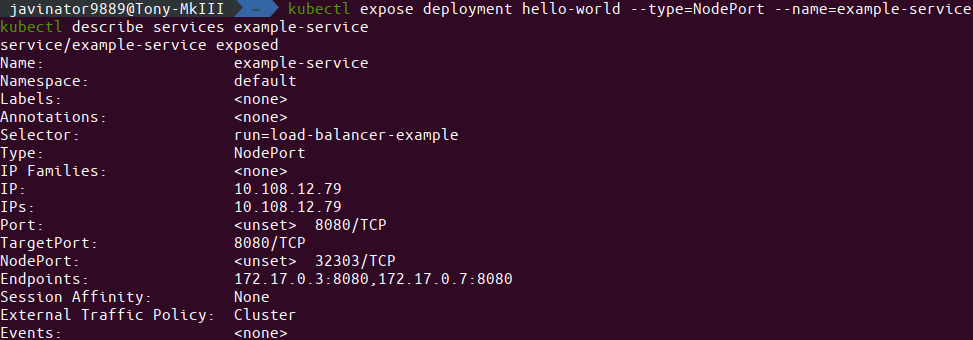
\includegraphics[width=.9\linewidth]{pictures/k8s-service.png}
    \caption{Información sobre el servicio recién desplegado de Kubernetes.}
    \label{fig:k8s-service}
\end{figure}

La salida anterior (imagen \ref{fig:k8s-service}) nos indica información sobre
lo que está en ejecución, el puerto de destino dentro del contenedor y el
puerto expuesto en el valor \texttt{NodePort}. Para comprobar que la aplicación
funciona, obtenemos la dirección IP del clúster de Kubernetes (comando
\lstinline[style=bash]!kubectl cluster-info!) y accedemos directamente desde
el navegador o desde el terminal, a la dirección \texttt{http://<node-ip>:<node-port>}
(figura \ref{fig:hello-k8s}):

\begin{figure}[H]
    \centering
    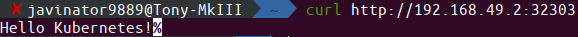
\includegraphics[width=.5\linewidth]{pictures/hello-kubernetes.png}
    \caption{El clúster de Kubernetes responde a nuestra petición web.}
    \label{fig:hello-k8s}
\end{figure}

\noindent\rule{\linewidth}{.2pt}

\subsubsection*{Docker Swarm}
